\documentclass[12pt]{article}

\setlength{\oddsidemargin}{20pt}
\setlength{\topmargin}{-30pt}
\setlength{\textwidth}{6in}
\setlength{\textheight}{640pt}

\setlength{\parindent}{0pt}
\setlength{\parskip}{10pt}



\newcommand{\outdate}{Saturday, March 4}
\newcommand{\duedate}{Friday, March 10, by 11:59 pm}

\newcommand{\codename}{\href{https://www.youtube.com/watch?v=LkMBvntR1cM}{... but maybe the printing press was heavier than the siege weapon}}

\renewcommand{\baselinestretch}{1.1}


\usepackage{ifthen}
\usepackage{pifont}
\usepackage{url}
\usepackage{hyperref}
\usepackage{graphicx}
\graphicspath{{figures/},{figures/local/}}

\usepackage{amsmath}
\usepackage{latexsym}
\usepackage{amssymb}
\usepackage{enumitem}
\usepackage{bbm}

\setlength{\columnseprule}{.5pt}


\newboolean{solutionsboolean}
\newboolean{videoboolean}

\urlstyle{same}

\usepackage{comment}

\usepackage[usenames]{color}
\newcommand{\tc}[2]{\textcolor{#1}{#2}}
\newcommand{\tcn}[2]{\color[named]{#1}{#2}}
\definecolor{olivegreen}{rgb}{0.33333,.41961,0.18431}
\definecolor{forestgreen}{rgb}{0.13333,.5451,0.13333}
\definecolor{lightgrey}{rgb}{0.7,0.7,0.7}
\definecolor{grey}{rgb}{0.5,0.5,0.5}
\definecolor{darkgrey}{rgb}{0.3,0.3,0.3}
\definecolor{verydarkgrey}{rgb}{0.1,0.1,0.1}

\usepackage{etoolbox}


\newcommand{\solutionstart}{\textbf{Solution:}}
\newcommand{\solutionend}{\hfill $\square$}

\usepackage{environ}

\NewEnviron{solution}{
  %% $\ulcorner$ \hfill $\urcorner$ \\

  \ifthenelse{\boolean{solutionsboolean}}{
    \normalcolor

    \solutionstart
    % \marginpar{\rule[-17.5mm]{1pt}{20mm}}
    \BODY
    \solutionend
  }

%%  \color{darkgrey}
  % $\llcorner$ \hfill $\lrcorner$ 
  % $\boxplus$
}[]




\usepackage{marvosym}

\newcommand{\pleasesubmitprojectdraft}{
  \ifthenelse{\not\boolean{solutionsboolean}}{
    {\small
    \textbf{Please submit your project's current draft}
    in pdf format via Blackboard by the same time specified for this assignment.
    For teams, please list all team member names clearly at the start.
%%     Please use this file name format (all lowercase after CSYS):\\
%%     \texttt{{\fullcoursenumbertext}project-\$firstname-\$lastname-YYYY-MM-DD.pdf}
%%     as in 
%%     \texttt{{\fullcoursenumbertext}project-lisa-simpson-1989-12-17.pdf}
%%     where the date is the date of submission (and not, say, your birthdate).
    }
    \medskip

    \hrule

    \medskip
  }{}
}

\usepackage{cancel}
\usepackage{verbatim}


\newcommand{\alert}[1]{#1}
\newcommand{\alertb}[1]{#1}


\newcommand{\tfline}{\underline{\mbox{\qquad \ }}.}


\newcommand{\veck}{\vec{k}}
%% \newcommand{\veck}{\mathbf{k}}

\newcommand{\infprob}{B}
\newcommand{\gainratio}{\mathbf{R}}

\newcommand{\undmark}{\rm und}
\newcommand{\dirmark}{\rm dir}

\newcommand{\bidmark}{\rm u}
\newcommand{\inmark}{\rm i}
\newcommand{\outmark}{\rm o}

\newcommand{\kin}{k_{\inmark}}
\newcommand{\kout}{k_{\outmark}}
\newcommand{\kbid}{k_{\bidmark}}

\newcommand{\jin}{j_{\inmark}}
\newcommand{\jout}{j_{\outmark}}
\newcommand{\jbid}{j_{\bidmark}}


\newcommand{\Probdir}{P^{(\rm \dirmark)}}

\newcommand{\Probin}{P^{(\rm \inmark)}}
\newcommand{\Probout}{P^{(\rm \outmark)}}
\newcommand{\Probbid}{P^{(\rm \bidmark)}}

\newcommand{\nodetype}{\kin,\kout,\kbid}

\newcommand{\edgetype}{\veck\, |\, \veck'}
\newcommand{\edgetypescript}{\veck\veck'}

%% \newcommand{\probfc}{\chi}
\newcommand{\probfc}{Q}

%% \newcommand{\edgetype}{\vec{k};\vec{\alpha}\, |\, \vec{k}';\vec{\alpha}'}
%% \newcommand{\edgetypescript}{\vec{k}\vec{\alpha}\vec{k}'\vec{\alpha}'}

\newcommand{\indrspfn}{h}
\newcommand{\rspfn}{H}

\newcommand{\solutioncolorswitch}{\color{darkgrey}}

%% \newcommand{\solution}[1]
%% {
%% % $\ulcorner$ \hfill $\urcorner$ \\
%% 
%% \normalcolor
%% 
%% \textbf{Solution:} 
%% % \marginpar{\rule[-17.5mm]{1pt}{20mm}}
%% \color{black}{#1}
%% % $\llcorner$ \hfill $\lrcorner$ 
%% % $\boxplus$
%% \hfill $\square$
%% 
%% \color{darkgrey}
%% 
%% }



\newcommand{\solutionsto}{Solutions to }

\setboolean{solutionsboolean}{true}
\setboolean{videoboolean}{false}

\newcommand{\assignmentsonly}[1]{}

\usepackage{media9}

\usepackage{censor}


%% set current time
\usepackage{datetime}
%% \yyyymmdddate
\newtimeformat{mytime}{\twodigit{\THEHOURXII}:\twodigit{\THEMINUTE}}
\settimeformat{mytime}
\newdateformat{mydate}{\dayofweekname{\THEDAY}{\THEMONTH}{\THEYEAR}, \monthname\ \THEDAY, \THEYEAR}
\mydate

%% for toggling solutions
\usepackage{environ}

%% eh
\newcommand{\pocsvoloneonly}[1]{}
\newcommand{\pocsvoltwoonly}[1]{}

%% links
\usepackage{url}
%% url style
\urlstyle{same}

%% allow hyphenation for urls with long many-hyphenated strings
\PassOptionsToPackage{hyphens}{url}\usepackage{hyperref}
\makeatletter
\g@addto@macro{\UrlBreaks}{\UrlOrds}
\makeatother

\usepackage{hyperref}
\hypersetup{
    colorlinks=true,
    linkcolor=grey,
    citecolor=todoblue,
    filecolor=grey,
    urlcolor=grey,
    breaklinks=true,
}

%% exciting emphasis action
\usepackage{ulem}
%% note that to allow linebreaking,
%% separate words as \dashuline{the\ slithy\ tove};
%% it may be necessary to format arguments 
%% in this way (e.g., section headings)
%% base html for documents (lectures and assignments)

\usepackage{cprotect}
%% code snippets
%% http://stackoverflow.com/questions/3175105/how-to-insert-code-into-a-latex-doc
\usepackage{listings}
\usepackage[numbered]{matlab-prettifier}

%% showing latex along with output
%% https://tex.stackexchange.com/questions/110349/any-way-to-show-latex-example-code-and-execute-it
\usepackage{showexpl}

%% use this for functions:
%% \begin{lstlisting}[style=Matlab-editor]
%% \end{lstlisting}\begin{verbatim}

\usepackage{fontawesome}


\definecolor{todoblue}{RGB}{0, 91, 187}
\newcommand{\todo}[1]{\noindent\textcolor{todoblue}{{$\Box$ #1}}}

\newcommand{\wikilink}[1]{\href{#1}{\tc{grey}{\faExternalLink}}}
\newcommand{\wordwikilink}[2]{\href{#1}{\tc{grey}{\dashuline{#2}~\faExternalLink}}}
\newcommand{\wordwikilinklong}[2]{\href{#1}{\tc{grey}{\url{#2}~\faExternalLink}}}



\newcommand{\Prob}{\mathbf{Pr}}

\newcommand{\degree}{\, \circ}
\newcommand{\tempf}[1]{${#1}^{\degree}F$}
\newcommand{\tempc}[1]{${#1}^{\degree}C$}

\newcommand{\avg}[1]{\left\langle#1\right\rangle}
\newcommand{\tavg}[1]{\langle#1\rangle}

\newcommand{\LavgHa}[2]{\tavg{L_{#1,#2}}}
\newcommand{\LavgHaN}[2]{\tavg{L_{#1,#2}}}
\newcommand{\Lavg}{\tavg{L}}

\newcommand{\sindex}[1]{}
\newcommand{\nindex}[1]{}

\newcommand{\etal}{\textit{et al.}}
\newcommand{\www}[1]{\url{#1}}
\newcommand{\req}[1]{(\ref{#1})}
\newcommand{\Req}[1]{Eq.~(\ref{#1})}


\newcommand{\yes}{}
\newcommand{\no}{}
\newcommand{\tbf}{\textbf}
\newcommand{\tit}{\textit}

\newcommand{\stirlingnumber}[2]{\genfrac{\{}{\}}{0pt}{}{#1}{#2}}


\newcommand{\dee}[1]{\mbox{d}#1}
\newcommand{\pdiff}[2]{\frac{\partial #1}{\partial #2}}
\newcommand{\partialdiff}[2]{\frac{\partial #1}{\partial #2}}
\newcommand{\partialdiffsq}[2]{\frac{\partial^2 #1}{\partial #2^2}}
\newcommand{\pdiffsq}[2]{\frac{\partial^2 #1}{{\partial #2}^2}}
\newcommand{\diff}[2]{\frac{{\rm d}#1}{{\rm d}#2}}
\newcommand{\diffsq}[2]{\frac{{\rm d}^{2}#1}{{\rm d} {#2}^2}}
\newcommand{\tdiff}[2]{\mbox{d} #1/\mbox{d} #2}
\newcommand{\tdiffsq}[2]{\mbox{d}^{2} #1/\mbox{d} {#2}^2}
\newcommand{\tpdiff}[2]{\partial #1/\partial #2}
\newcommand{\tpdiffsq}[2]{\partial^2 #1/\partial {#2}^2}
\newcommand{\postdee}[1]{\,\mbox{d}#1}


%% binomials
\newcommand{\mybinom}[2]{\Bigl(\begin{array}{@{}c@{}}#1\\#2\end{array}\Bigr)}

%% half
\newcommand{\half}{\frac{1}{2}}



% \newcommand{\avgSL}{\bar{L}_{\rm s}}
\newcommand{\avgSL}{\tavg{l_{\rm s}}}


\newcommand{\fplus}{f_{+}}
\newcommand{\fminus}{f_{-}}
\newcommand{\aplus}{a_{+}}
\newcommand{\aminus}{a_{-}}



% \newcommand{\kstar}{d^{\ast}}
% \newcommand{\kstari}{k_i^\ast}
\newcommand{\kstar}{d^\ast}
\newcommand{\kstari}{d_i^\ast}

\newcommand{\dstar}{d^\ast}
\newcommand{\dstari}{d_i^\ast}

\newcommand{\phifix}{{\phi^{\ast}}}
\newcommand{\phifixc}{{\phi_c^{\ast}}}
\newcommand{\phifixb}{{\phi_b^{\ast}}}

\newcommand{\Gfun}{G}


\newcommand{\dstardist}{g}
\newcommand{\dosedist}{f}
\newcommand{\dosedistk}{f^{k\star}}

\newcommand{\erdosrenyi}{Erd\"{o}s-R\'{e}nyi}

\newcommand{\meandegree}{z}

\newcommand{\stateA}{0}
\newcommand{\stateB}{1}

\newcommand{\phiA}{\phi_0}
\newcommand{\phiB}{\phi_1}

\newcommand{\phiup}{\phi^{\rm up}}
\newcommand{\phidown}{\phi^{\rm down}}
\newcommand{\phiupi}{\phi_i^{\rm up}}
\newcommand{\phidowni}{\phi_i^{\rm down}}

\newcommand{\phihomog}{\phi_{\rm h}}
\newcommand{\phiuphomog}{\phi_{\rm h}^{\rm up}}

\newcommand{\vcluster}{\mathcal{V}_{\rm max}}
\newcommand{\initset}{\mathcal{A}}

\newcommand{\avggroupdeg}{\tavg{k_{\rm group}}}

\newenvironment{packed_enum}{
\begin{enumerate}
  \setlength{\itemsep}{1pt}
  \setlength{\parskip}{0pt}
  \setlength{\parsep}{0pt}
}{\end{enumerate}}


%% scaling

\newcommand{\xmin}{x_\textnormal{min}}
\newcommand{\xmax}{x_\textnormal{max}}


%% video hints:

\newcommand{\videohint}[2]{
  \ifthenelse{\boolean{videoboolean}}{
 \begin{minipage}{1.0\linewidth}
   \textbf{Hint---}#2:\\
   \includemedia[
   width=1\linewidth,height=0.5625\linewidth,
   activate=pageopen,
   flashvars={
     modestbranding=0 % no YT logo in control bar
     &autoplay=0
     &fs=1
     &autohide=1 % controlbar autohide
     &showinfo=0 % no title and other info before start
     % &rel=0
     % &rel=0 % no related videos after end
   }
   ]
   {}
   {http://www.youtube.com/watch?v=#1}\\
   Direct link: \url{http://www.youtube.com/watch?v=#1}
%   {http://www.youtube.com/watch?v=#1?rel=0}\\
%   Direct link: \url{http://www.youtube.com/watch?v=#1?rel=0}
   %% \url{http://www.youtube.com/watch?v=#1?rel=0}
 \end{minipage}
  }
  {
    \textbf{Hint---#2}: \url{http://www.youtube.com/watch?v=#1}
%%    \textbf{Hint---#2}: \url{http://www.youtube.com/watch?v=#1?rel=0}
  }
}

\newcommand{\videohelp}[7]{
  %% youtube embeds no longer work
  %% 
%%   %% #1: video
%%   %% #2: title
%%   %% #3: start
%%   %% #4: end (only works in embed)
%%   %% #5: video length
  \ifthenelse{\boolean{videoboolean}}{
    \begin{minipage}{1.0\linewidth}
      \textbf{Help---}#2 (runs from #5 to #6, length #7):\\
      \includemedia[
      width=1\linewidth,height=0.5625\linewidth,
      activate=pageopen,
      flashvars={
        modestbranding=0 % no YT logo in control bar
        &autoplay=0
        &fs=1
        &autohide=0 % controlbar autohide
        &showinfo=0 % no title and other info before start
        &start=#3
        &end=#4
%        &rel=0
        % &rel=0 % no related videos after end
      }
      ]
      {}
      %% {http://www.youtube.com/watch?v=#1?rel=0&start=#3&end=#4}\\
      {http://www.youtube.com/watch?v=#1?start=#3&end=#4}\\
      \tc{grey}{Note: Video embed only works in Adobe Reader. Direct link:}\\
      \tc{grey}{\url{http://www.youtube.com/watch?v=#1?\&start=#3\&end=#4}}
%%      \tc{grey}{\url{http://www.youtube.com/watch?v=#1\&rel=0\&start=#3\&end=#4}}
      %% \url{http://www.youtube.com/watch?v=#1?start=#3&end=#4&rel=0}
    \end{minipage}
  }
  {
    \textbf{Help---#2} (runs from #5 to #6, length #7): \url{http://www.youtube.com/watch?v=#1?start=#3\&end=#4}
%%    \textbf{Help---#2} (runs from #5 to #6, length #7): \url{http://www.youtube.com/watch?v=#1\?rel=0\&start=#3\&end=#4}
  }
}


%%%%%%%%%%%%%%%%%%%%%%%%%%%%%%%%%%%%%%%%%%%%%%%%%%%%%%
%% matrices
%%%%%%%%%%%%%%%%%%%%%%%%%%%%%%%%%%%%%%%%%%%%%%%%%%%%%%

\newcommand{\m}[1]{\mathbf{#1}}

\newcommand{\colvec}[1]{
\left[
  \begin{array}{c}
    #1
  \end{array}
\right]
}

\newcommand{\rowop}[3]{
  {
    \scriptsize
    \begin{array}{c}
      \mbox{\Large $\leadsto$} \\
      \mbox{#1' =} \\
      \mbox{#1 -} \\ 
      \mbox{#2 #3} \\
    \end{array}
  }
}

\newcommand{\rowoptwobytwo}[3]{
  {
    \scriptsize
    \begin{array}{c}
      \mbox{\Large $\leadsto$} \\
      \mbox{#1'} 
      \mbox{= #1 -}
      \mbox{#2 #3} \\
    \end{array}
  }
}

\newcommand{\rowopeq}[3]{
  {
    \scriptsize
    \begin{array}{c}
      \mbox{\Large =} \\
      \left\lgroup
      \mbox{\tiny
        \begin{tabular}{c}
          #1' =  \\
          #1 - #2 #3 \\
        \end{tabular}
    }
      \right\rgroup
    \end{array}
  }
}

\newcommand{\rowswapeq}[2]{
  {
    \scriptsize
    \begin{array}{c}
      \mbox{\large =} \\
      \left\lgroup
      \mbox{\tiny
          #1 $\leftrightarrow$ #2
        }
      \right\rgroup
    \end{array}
  }
}

\newcommand{\rowdiv}[2]{
  {
    \scriptsize
    \begin{array}{c}
      \mbox{\Large $\leadsto$} \\
      \mbox{#1' =} \\
      \mbox{#1/(#2)} \\ 
    \end{array}
  }
}

\newcommand{\rowdivthreebythree}[3]{
  {
    \scriptsize
    \begin{array}{c}
      \mbox{\Large $\leadsto$} \\
      \mbox{row 1'} = \mbox{row 1/(#1)}\\
      \mbox{row 2'} = \mbox{row 2/(#2)}\\
      \mbox{row 3'} = \mbox{row 3/(#3)}\\
    \end{array}
  }
}


\newcommand{\rowdivtwobytwo}[2]{
  {
    \scriptsize
    \begin{array}{c}
      \mbox{\Large $\leadsto$} \\
      \mbox{row 1'} = \mbox{row 1/(#1)}\\
      \mbox{row 2'} = \mbox{row 2/(#2)}\\
    \end{array}
  }
}

\newcommand{\rowdivtwobytwoeq}[2]{
  {
    \scriptsize
    \begin{array}{c}
      \mbox{\Large =} \\
      \mbox{row 1'} = \mbox{row 1/(#1)}\\
      \mbox{row 2'} = \mbox{row 2/(#2)}\\
    \end{array}
  }
}

\newcommand{\rowdivthreebythreeeqR}[3]{
  {
    \scriptsize
    \begin{array}{c}
      \mbox{\Large =} \\
      \mbox{R1'} = \mbox{R1/(#1)}\\
      \mbox{R2'} = \mbox{R2/(#2)}\\
      \mbox{R3'} = \mbox{R3/(#3)}\\
    \end{array}
  }
}


\newcommand{\rowdivtwobytwoeqR}[2]{
  {
    \scriptsize
    \begin{array}{c}
      \mbox{\Large =} \\
      \mbox{R1'} = \mbox{R1/(#1)}\\
      \mbox{R2'} = \mbox{R2/(#2)}\\
    \end{array}
  }
}


\newcommand{\rowonediv}[1]{
  {
    \scriptsize
    \begin{array}{c}
      \mbox{\Large $\leadsto$} \\
      \mbox{row 1'} = \mbox{row 1/#1}\\
    \end{array}
  }
}

\newcommand{\mymatrix}[2]{
  \left[
  \begin{array}{#1}
    #2
  \end{array}
  \right]
}

%% \newcommand{\matrix}[1]{\mathbf{#1}}
\newcommand{\textmatrix}[1]{#1}

%% \renewcommand{\m}[1]{\mathbf{#1}}

\newcommand{\Axb}{\textmatrix{A}\vec{x}=\vec{b}}
\newcommand{\Axzero}{\textmatrix{A}\vec{x}=\vec{0}}
\newcommand{\A}{\textmatrix{A}}
\newcommand{\AT}{\textmatrix{A}^{\rm T}}
\newcommand{\CA}{C(\textmatrix{A})}
\newcommand{\NA}{N(\textmatrix{A})}
\newcommand{\CAT}{C(\textmatrix{A}^{\rm T})}
\newcommand{\NAT}{N(\textmatrix{A}^{\rm T})}

\newcommand{\I}{\textmatrix{I}}
\newcommand{\R}{\textmatrix{R}}

\newcommand{\augAb}{[\A \, | \, \vec{b} \, ]}

\newcommand{\rref}[1]{\R_{#1}}

\newcommand{\lmat}{\left[
\begin{array}
}
\newcommand{\rmat}{\end{array}
\right]
}



%% girl born on a tuesday problem
\newcommand{\girl}{G}
\newcommand{\boy}{B}
\newcommand{\girltues}{G_{\textnormal{Tue}}}


%% entropy
\newcommand{\Hrenyi}[1]{H^{\textnormal{(R)}}_{#1}}
\newcommand{\Htsallis}[1]{H^{\textnormal{(T)}}_{#1}}
%% branching networks

%% river networks
\newcommand{\rhodd}{\rho_{\rm dd}} % drainage density
\newcommand{\msl}{\ell} % main stream length
%% \newcommand{\okell}{{l^{\mbox{\scriptsize{(s)}}}}}
%% \newcommand{\okellsnum}[1]{l_{#1}^{\mathrm{\, (s)}}}
\newcommand{\okell}{s}
\newcommand{\okellsnum}[1]{s_{#1}}

\newcommand{\om}{\omega}
\newcommand{\Om}{\Omega}

\newcommand{\Tmunu}{T_{\mu,\nu}}

\newcommand{\rpartition}[7]{%
  #1(#2\!\!#3,#4\!\!#5#6#7)}

%%%%%%%%%%%%%%%%%%%%%%%%%%%%%%%%%%%
%% optimal forks (Murray's law)
%%%%%%%%%%%%%%%%%%%%%%%%%%%%%%%%%%%

\newcommand{\rparent}{r_{\textnormal{parent}}}
\newcommand{\rchilda}{r_{\textnormal{offspring} 1}}
\newcommand{\rchildb}{r_{\textnormal{offspring} 2}}

%%%%%%%%%%%%%%%%%%%%%%%%%%%%%%%%%%%
%% optimal supply networks
%%%%%%%%%%%%%%%%%%%%%%%%%%%%%%%%%%%

\newcommand{\rhofac}{\rho_{\textnormal{fac}}}
\newcommand{\rhopop}{\rho_{\textnormal{pop}}}

%% supply networks

\newcommand{\volume}[1]{\Omega_{d,D}(#1)}

\newcommand{\vnet}{V_{\rm net}}

%% chaotic contagion

\newcommand{\niprob}{q}
\newcommand{\liprob}{r}


%% random biparite networks

\newcommand{\rbone}{\textnormal{\faFilm}}
\newcommand{\rbtwo}{\textnormal{\faLightbulbO}}

\newcommand{\rboneng}{N_{\rbone}}
\newcommand{\rbtwong}{N_{\rbtwo}}

\newcommand{\Prboneind}{P^{(\rbone)}_{\textnormal{ind},k}}
\newcommand{\Prbtwoind}{P^{(\rbtwo)}_{\textnormal{ind},k}}

\newcommand{\Rrboneind}{R^{(\rbone)}_{\textnormal{ind},k}}
\newcommand{\Rrbtwoind}{R^{(\rbtwo)}_{\textnormal{ind},k}}

\newcommand{\Prboneindplain}{P^{(\rbone)}_{\textnormal{ind}}}
\newcommand{\Prbtwoindplain}{P^{(\rbtwo)}_{\textnormal{ind}}}

\newcommand{\Rrboneindplain}{R^{(\rbone)}_{\textnormal{ind}}}
\newcommand{\Rrbtwoindplain}{R^{(\rbtwo)}_{\textnormal{ind}}}

%%%%%%%%%%%%%%%%%%%%%%%%%%%%%%%%%%%%%%%%%%%%%%%%%%%%%%%%%%%%%%%%%
%% happiness

\newcommand{\havg}[1]{h_{\rm avg}(#1)}
\newcommand{\havgword}[1]{h_{\rm avg}(\textnormal{`#1'})}
\newcommand{\havgsup}[1]{h_{\rm avg}^{#1}}
\newcommand{\havgsuparg}[2]{h_{\rm avg}^{#1}(#2)}

\newcommand{\havgfn}{h_{\rm avg}}
\newcommand{\hstdfn}{h_{\textnormal{std}}}

\newcommand{\havgfnamb}{h_{\rm avg}^{\rm (amb)}}
\newcommand{\havgfnnorm}{h_{\rm avg}^{\rm (norm)}}


\newcommand{\Tref}{T_{\textnormal{ref}}}
\newcommand{\Tcomp}{T_{\textnormal{comp}}}

\newcommand{\deltahw}{\delta_{h}(w)}
\newcommand{\deltapw}{\delta_{p}(w)}



%% contagion
\newcommand{\vuln}{\textnormal{vuln}}
\newcommand{\trig}{\textnormal{trig}}
\newcommand{\Svuln}{S_{\textnormal{vuln}}}
\newcommand{\thetavuln}{\theta_{\textnormal{vuln}}}
\newcommand{\Strig}{S_{\textnormal{trig}}}
\newcommand{\Ptrig}{P_{\textnormal{trig}}}
\newcommand{\Sgc}{S_{\textnormal{gc}}}

\newcommand{\emn}{e_{\mu\nu}}
\newcommand{\emm}{e_{\mu\mu}}
\newcommand{\exx}{e_{x y}}
\newcommand{\exy}{e_{x x}}
\newcommand{\ejk}{e_{j k}}
\newcommand{\ejj}{e_{j j}}
\newcommand{\ekj}{e_{k j}}

%%%%%%%%%%%%%%%%%%%%%%%%%%%%%%%%%%%
%% 80/20 rule, Gini coefficient
%%%%%%%%%%%%%%%%%%%%%%%%%%%%%%%%%%%

\newcommand{\fracsymbol}{\theta}
\newcommand{\popfrac}{\fracsymbol_{\textnormal{pop}}}
\newcommand{\wealthfrac}{\fracsymbol_{\textnormal{wealth}}}
\newcommand{\ginicoefficient}{G}


%%%%%%%%%%%%%%%%%%%%%%%%%%%%%%%%%%%
%% Zipf, Simon's scaling
%%%%%%%%%%%%%%%%%%%%%%%%%%%%%%%%%%%

%% simon's model
\newcommand{\simonalpha}{\rho}

\newcommand{\simonrho}{\rho}
%% \newcommand{\zipfrank}{r}
%% \newcommand{\zipfexponent}{\alpha}
%% \newcommand{\frequency}{f}
\newcommand{\probsymbol}{p}
\newcommand{\zipfrankmax}{\zipfrank_{\textnormal{max}}}


%% rank for Zipf's law
\newcommand{\rank}{r}

%% rich gets richer model

%% same as simonrho

\newcommand{\zipfrank}{r}
\newcommand{\zipfexponent}{\alpha}

\newcommand{\groupnum}{n}

\newcommand{\innovationrate}{\rho}
\newcommand{\innovationratet}{\rho_{t}}

\newcommand{\rgrN}{S}
\newcommand{\Ngroups}{N}

%% \newcommand{\rgrNt}[1]{\rgrN_{#1}^{\textnormal{(e)}}}
%% \newcommand{\rgrNinit}{\rgrN^{\textnormal{(e,\textnormal{init})}}}
\newcommand{\rgrNt}[1]{\rgrN_{#1}}
\newcommand{\rgrNinit}{\rgrN^{\textnormal{\textnormal{init}}}}

\newcommand{\grouptimestart}[1]{t_{#1}^{\textnormal{init}}}

\newcommand{\groupsizet}[2]{\rgrN_{#1,#2}}
%% \newcommand{\groupsizet}[2]{\rgrN_{#1,#2}^{\textnormal{(e)}}}
%% \newcommand{\groupsizet}[2]{\rgrN_{#1}^{\textnormal{(e)}}(#2)}

\newcommand{\groupnumt}[1]{\Ngroups^{\textnormal{(g)}}_{#1}}

\newcommand{\rgrP}{P}
\newcommand{\groupprobt}[2]{\rgrP_{#1,#2}}
%% \newcommand{\groupprobt}[2]{\rgrP_{#1,#2}^{\textnormal{(e)}}}

\newcommand{\Beta}{B}

\newcommand{\onehalf}{\frac{1}{2}}
\newcommand{\onequarter}{\frac{1}{4}}


%% \newcommand{\Ngroupsinit}{\Ngroups_{\textnormal{init}}}
\newcommand{\groupnuminit}{\groupnum^{\textnormal{init}}}

%% language, lexical turbulence

%% language, zipf
\newcommand{\frequency}{f}

\newcommand{\frequencythreshold}{f_{\textnormal{thr}}}
%% \newcommand{\frequencythreshold}{f_{\Asterisk}}

\newcommand{\frequencyword}{f_{w;y}}
\newcommand{\frequencymedian}[2]{f_{w;#1,#2}^{\textnormal{med}}}
\newcommand{\frequencycut}[2]{f_{w;#1,#2}^{\textnormal{cut}}}


\newcommand{\flux}{\phi}
\newcommand{\fluxup}{\flux_{\textnormal{up}}}
\newcommand{\fluxdown}{\flux_{\textnormal{down}}}

\newcommand{\zipfexponentlower}{\alpha}
\newcommand{\zipfexponentupper}{\alpha'}

\newcommand{\fluxexponentlower}{\mu}
\newcommand{\fluxexponentupper}{\mu'}

\newcommand{\fluxrankexponentlower}{\nu}
\newcommand{\fluxrankexponentupper}{\nu'}

\newcommand{\breakpoint}{\textnormal{b}}
\newcommand{\zipfbreakpoint}{\zipfrank_{\breakpoint}}
%% \newcommand{\frequencythresholdbreakpoint}{{\frequencythreshold}_{,\textnormal{b}}}
\newcommand{\frequencythresholdbreakpoint}{f_{\breakpoint}}
 


%%%%%%%%%%%%%%%%%%%%%%%%%%%%%%%%%%%
%% allotaxonometry:
%% 
%% universal categorical data shifts
%% 
%% - general 
%%%%%%%%%%%%%%%%%%%%%%%%%%%%%%%%%%%

\newcommand{\sizesymbol}{s}
\newcommand{\numbersymbol}{N}
\newcommand{\bigprobsymbol}{P}
\newcommand{\bigrank}{R}

\newcommand{\indexaraw}{1}
\newcommand{\indexbraw}{2}

\newcommand{\indexa}{(\indexaraw)}
\newcommand{\indexb}{(\indexbraw)}
\newcommand{\indexavg}{(\indexaraw\cdot\indexbraw)}

\newcommand{\indexref}{\textnormal{(ref)}}

\newcommand{\indexanyraw}{i}
\newcommand{\indexany}{(\indexanyraw)}

\newcommand{\measuresymbol}{\phi}
\newcommand{\bigmeasuresymbol}{\Phi}


\newcommand{\systemsymbol}{\Omega}
\newcommand{\elementsymbol}{\tau}

\newcommand{\elementsetsymbol}{\mathcal{T}}
\newcommand{\elementsetsymbola}{\mathcal{T}^{\indexa}}
\newcommand{\elementsetsymbolb}{\mathcal{T}^{\indexb}}
\newcommand{\elementsetsymbolany}{\mathcal{T}^{\indexany}}

\newcommand{\systema}{\systemsymbol^{\indexa}}
\newcommand{\systemb}{\systemsymbol^{\indexb}}
\newcommand{\systemavg}{\systemsymbol^{\indexavg}}
\newcommand{\systemref}{\systemsymbol^{\indexref}}
\newcommand{\systemany}{\systemsymbol^{\indexany}}

\newcommand{\Ntypesa}{\numbersymbol_{\indexaraw}}
\newcommand{\Ntypesb}{\numbersymbol_{\indexbraw}}
%% \newcommand{\Ntypesa}{\numbersymbol_{\systema}}
%% \newcommand{\Ntypesb}{\numbersymbol_{\systemb}}

\newcommand{\sizea}{\sizesymbol^{\indexa}}
\newcommand{\sizeb}{\sizesymbol^{\indexb}}
\newcommand{\sizeany}{\sizesymbol^{\indexany}}

\newcommand{\texta}{\textsymbol^{\indexa}}
\newcommand{\textb}{\textsymbol^{\indexb}}
\newcommand{\textany}{\textsymbol^{\indexany}}

\newcommand{\numbera}{\numbersymbol^{\indexa}}
\newcommand{\numberb}{\numbersymbol^{\indexb}}
\newcommand{\numberany}{\numbersymbol^{\indexany}}

\newcommand{\proba}{\probsymbol^{\indexa}}
\newcommand{\probb}{\probsymbol^{\indexb}}
\newcommand{\probavg}{\probsymbol^{\indexavg}}
\newcommand{\probany}{\probsymbol^{\indexany}}

\newcommand{\probmixedab}{\probsymbol^{(\indexaraw,\indexbraw)}}

\newcommand{\measurea}{\measuresymbol^{\indexa}}
\newcommand{\measureb}{\measuresymbol^{\indexb}}
\newcommand{\measureavg}{\measuresymbol^{\indexavg}}
\newcommand{\measureany}{\measuresymbol^{\indexany}}
\newcommand{\measureref}{\bigmeasuresymbol_{\systemref}}

%%%%%%%%%%%%%%%%%%%%%%%%%%%%%%%%%%%
%% Entropy, Divergences
%%%%%%%%%%%%%%%%%%%%%%%%%%%%%%%%%%%

\newcommand{\diffsummand}{\delta\bigmeasuresymbol_{\elementsymbol}(\systemb,\systema)}


%%%%%%%%%%%%%%%%%%%%%%%%%%%%%%%%%%%
%% rank divergence
%%%%%%%%%%%%%%%%%%%%%%%%%%%%%%%%%%%

\newcommand{\rtd}[1]{D^{\textnormal{R}}_{#1}}
\newcommand{\rtdelement}[1]{\delta D^{\textnormal{R}}_{#1,\elementsymbol}}

\newcommand{\rtdhalf}{\rtd{\sfrac{1}{2}}}
\newcommand{\rtdhalfelement}{\rtdelement{\sfrac{1}{2}}}

\newcommand{\rtdalpha}{\rtd{\alpha}}
\newcommand{\rtdalphaelement}{\rtdelement{\alpha}}

%% alpha as a variable
\newcommand{\rtdalphavar}[1]{\rtd{#1}}
\newcommand{\rtdalphavarelement}[1]{\rtdelement{#1}}

%% \newcommand{\rtdnorm}{C_{\textnormal{\bigrank}}}
%% \newcommand{\rtdnorm}{\mathcal{N}_{\textnormal{\bigrank}}}
%% \newcommand{\rtdnorm}{\mathcal{N}_{\bigrank_{\indexaraw,\indexbraw;\alpha}}}
\newcommand{\rtdnorm}{\mathcal{N}_{\indexaraw,\indexbraw;\alpha}}
\newcommand{\invrtdnorm}{\frac{1}{\rtdnorm}}

\newcommand{\rtdnormalpha}[1]{\mathcal{N}_{\indexaraw,\indexbraw;#1}}
\newcommand{\invrtdnormalpha}[1]{\frac{1}{\rtdnormalpha{#1}}}

\newcommand{\rtdalphasystems}[2]{\rtdalpha(#1\,\|\,#2)}
\newcommand{\rtdalphasystemsOmega}{\rtdalphasystems{\systemsymbol_{\indexaraw}}{\systemsymbol_{\indexbraw}}}
\newcommand{\rtdalphasystemsRank}{\rtdalphasystems{\bigrank_{\indexaraw}}{\bigrank_{\indexbraw}}}
\newcommand{\rtdalphasystemsRankRand}{\rtdalphasystems{\bigrank_{\indexaraw}}{\bigrank_{\indexbraw}}}

\newcommand{\rtdalphavarsystems}[3]{\rtdalphavar{#1}(#2\,\|\,#3)}
\newcommand{\rtdalphavarsystemsOmega}[1]{\rtdalphavarsystems{#1}{\systemsymbol_{\indexaraw}}{\systemsymbol_{\indexbraw}}}
\newcommand{\rtdalphavarsystemsRank}[1]{\rtdalphavarsystems{#1}{\bigrank_{\indexaraw}}{\bigrank_{\indexbraw}}}

\newcommand{\rtdalphavarsystemsRankRand}[1]{\rtdalphavarsystems{#1; \textnormal{rand}}
   {\bigrank_{\indexaraw}}
   {\bigrank_{\indexbraw}}}

%% \newcommand{\rtdalphavarsystemsRankRand}[1]{D^{\textnormal{R,rand}}_{#1}
%%  (\bigrank_{\indexaraw}\,\|\,\bigrank_{\indexbraw})}

%% merged systems, ordering of contributions for rank probability
\newcommand{\bigrankordering}{\bigrank_{\indexaraw,\indexbraw;\alpha}}
\newcommand{\bigrankorderingalpha}[1]{\bigrank_{\indexaraw,\indexbraw;#1}}

%%%%%%%%%%%%%%%%%%%%%%%%%%%%%%%%%%%
%% probability divergence
%%%%%%%%%%%%%%%%%%%%%%%%%%%%%%%%%%%

\newcommand{\probdiv}[1]{D^{\textnormal{P}}_{#1}}
\newcommand{\probdivelement}[1]{D^{\textnormal{P}}_{#1,\elementsymbol}}

\newcommand{\probdivhalf}{\probdiv{\sfrac{1}{2}}}
\newcommand{\probdivhalfelement}{\probdivelement{\sfrac{1}{2}}}

\newcommand{\probdivalpha}{\probdiv{\alpha}}
\newcommand{\probdivalphaelement}{\probdivelement{\alpha}}

%% normalization factor

\newcommand{\ptdnorm}{\mathcal{N}_{\indexaraw,\indexbraw;\alpha}^{\textnormal{P}}}
\newcommand{\invptdnorm}{\frac{1}{\ptdnorm}}

\newcommand{\ptdnormalpha}[1]{\mathcal{N}_{\indexaraw,\indexbraw;#1}^{\textnormal{P}}}
\newcommand{\invptdnormalpha}[1]{\frac{1}{\ptdnormalpha{#1}}}

%%%%%%%%%%%%%%%%%%%%%%%%%%%%%%%%%%%
%% generalized entropy divergence
%%%%%%%%%%%%%%%%%%%%%%%%%%%%%%%%%%%

\newcommand{\gendiv}[1]{D^{\textnormal{AS2}}_{#1}}

%%%%%%%%%%%%%%%%%%%%%%%%%%%%%%%%%%%
%% jensen-shannon divergence
%%%%%%%%%%%%%%%%%%%%%%%%%%%%%%%%%%%

\newcommand{\jsd}{D^{\textnormal{JS}}}
\newcommand{\kld}{D^{\textnormal{KL}}}

\newcommand{\jsdelement}{D^{\textnormal{JS},\elementsymbol}}
\newcommand{\kldelement}{D^{\textnormal{KL},\elementsymbol}}

%%%%%%%%%%%%%%%%%%%%%%%%%%%%%%%%%%%
%% universal categorical data shifts
%% texts
%%%%%%%%%%%%%%%%%%%%%%%%%%%%%%%%%%%

\newcommand{\textsymbol}{T}

\newcommand{\logtwo}{\textnormal{log}_2}




\newcommand{\assignmentnum}{21}
\newcommand{\assignmentnumtext}{21}

\begin{document}

\setcounter{page}{1}

\raggedright

\sffamily

%% \solutioncolorswitch

%% volume one and two switches throughout

\newcommand{\coursename}{Principles of Complex Systems, Vols. 1, 2, \& 3D}
\newcommand{\courseacronym}{PoCS}
\newcommand{\courseuniverse}{The PoCSverse}
\newcommand{\courseacronymlc}{pocs}
\newcommand{\courseacronymcompact}{PoCS}
\newcommand{\coursetag}{pocsverse}
\newcommand{\fullcoursenumber}{CSYS/MATH 300, 303, \& 394}

\newcommand{\coursenamevolumeone}{Principles of Complex Systems}
\newcommand{\coursenamevolumetwo}{Complex Networks}
\newcommand{\coursenamevolumethree}{Principles of Complex Systems 3}
%% \newcommand{\coursenamevolumethree}{Advanced Topics in Complex Systems}
%% \newcommand{\coursenamevolumethree}{Advanced Topics in Complex Systems: Ousiometrics, Telegnomics, and Stories}

\newcommand{\coursenamevolumeoneshort}{Principles Complex Systems 1}
\newcommand{\coursenamevolumetwoshort}{Principles Complex Systems 2}
\newcommand{\coursenamevolumethreeshort}{Principles Complex Systems 3}


\newcommand{\coursenumber}{300}
\newcommand{\coursesection}{A}
\newcommand{\computernumber}{94574/96436/95291/96116}
\newcommand{\fullcoursenumbertext}{CSYS\coursenumber}

\newcommand{\coursenumbervolumeone}{300}
\newcommand{\coursesectionvolumeone}{A}
\newcommand{\computernumbervolumeone}{94574/96436/95291/96116}
\newcommand{\fullcoursenumbertextvolumeone}{CSYS\coursenumber}

\newcommand{\coursenumbervolumetwo}{303}
\newcommand{\coursesectionvolumetwo}{A}
\newcommand{\computernumbervolumetwo}{15321/15302}
\newcommand{\fullcoursenumbertextvolumetwo}{CSYS\coursenumbervolumetwo}

\newcommand{\coursenumbervolumethree}{394}
\newcommand{\coursesectionvolumethree}{A}
\newcommand{\computernumbervolumethree}{96364}
\newcommand{\fullcoursenumbertextvolumethree}{CSYS\coursenumbervolumethree}

\newcommand{\courseseason}{18}

\newcommand{\pocsvoltwostartassignment}{15}

%% %% vestigial
%% %% randomizer for course nickname
%% \perlnewcommand{\coursenickname}{
%%   @nicknames = ('Complex Networks: Revenge of the PoCS',
%%   'PoCS: Complex Networks Edition',
%%   'CocoNuTS',
%%   'CoNKs',
%%   'sCoNes',
%%   'Complex Networks: The PoCS Strikes Back',
%%   'Monk owl excerpts',
%%   'Next PoCS: Elk Worm',
%%   'Ex-crow pelts monk',
%%   'Plot: Corms Knew Ex',
%%   'Plot: Ex mocks Wren',
%%   'Plot: Ox wrecks men',
%%   );
%%   return $nicknames[rand @nicknames];
%% }

%% for assignments
\newcommand{\overleafurl}{https://www.overleaf.com/read/ppbnjdwpwttn}

\newcommand{\teamsurl}{https://teams.microsoft.com/l/channel/19\%3a4d62bc9c659c4717a884f02b54546f8d\%40thread.tacv2/General?groupId=24e0c156-f786-4d99-bbdd-5d4489db90e7\&tenantId=1c177758-4d6b-43dc-aaeb-3b9c42562967}
\newcommand{\slackurl}{}

\newcommand{\teamsurlsemesterone}{}
\newcommand{\teamsurlsemestertwo}{}

\newcommand{\courseyear}{2022}
\newcommand{\coursemonth}{08}
\newcommand{\season}{Fall}

\newcommand{\courseyearfirsthalf}{2022}
\newcommand{\coursemonthfirsthalf}{08}
\newcommand{\seasonfirsthalf}{Fall}

\newcommand{\courseyearsecondhalf}{2023}
\newcommand{\coursemonthsecondhalf}{01}
\newcommand{\seasonsecondhalf}{Spring}

\newcommand{\courseyearthirdhalf}{2022}
\newcommand{\coursemonththirdhalf}{08}
\newcommand{\seasonthirdhalf}{Fall}

\newcommand{\secondhalffirstassignmentnum}{15}

\newcommand{\lastcourseyear}{2021}
\newcommand{\lastcoursemonth}{08}

\newcommand{\logosuffix}{logo.pdf}
\newcommand{\courselogo}{\courseacronymlc\logosuffix}

\newcommand{\lectureroom}{Perkins 003}
\newcommand{\meetingtimes}{10:05 am to 11:20 am}
\newcommand{\lecturestarttime}{10:05 am}

\newcommand{\lectureroomvolumeone}{Perkins 003}
\newcommand{\meetingtimesvolumeone}{10:05 am to 11:20 am}
\newcommand{\lecturestarttimevolumeone}{10:05 am}

\newcommand{\lectureroomvolumetwo}{TBA}
\newcommand{\meetingtimesvolumetwo}{TBA}
\newcommand{\lecturestarttimevolumetwo}{TBA}

\newcommand{\lectureroomvolumethree}{TBA}
\newcommand{\meetingtimesvolumethree}{TBA}
\newcommand{\lecturestarttimevolumethree}{TBA}

\newcommand{\fullinstitution}{University of Vermont}
\newcommand{\institution}{UVM}

\newcommand{\coursehandle}{@pocsvox}
\newcommand{\coursetwitterhandlelink}{\href{https://twitter.com/\coursehandle}{\coursehandle}}
\newcommand{\coursehashtag}{\#\season\courseacronymcompact\courseyear}


\newcommand{\courseprefix}{\courseyearfirsthalf-\courseyearsecondhalf\coursetag}


%% websites
\newcommand{\institutionwebsite}{https://pdodds.w3.uvm.edu}
\newcommand{\mywebsitehomedir}{}

%% \newcommand{\visitinginstitutionwebsite}{http://www.massmutual.com}

%% \newcommand{\mywebsitehomedirtext}{$\sim$pdodds}
%% \newcommand{\mywebsitehomedirtext}{{\textasciitilde{}}pdodds}
\newcommand{\mywebsitehomedirtext}{}


\newcommand{\mywebsite}{\institutionwebsite/\mywebsitehomedir}
\newcommand{\mywebsiteresearch}{\institutionwebsite/research}
\newcommand{\mywebsitevideos}{\institutionwebsite/videos}
\newcommand{\myemailaddress}{peter.dodds+pocs@uvm.edu}
\newcommand{\mytwitterhandle}{@peterdodds}
\newcommand{\mytwitterhandlelink}{\href{https://twitter.com/\mytwitterhandle}{\mytwitterhandle}}

\newcommand{\teachingsite}{\institutionwebsite/teaching}
\newcommand{\coursewebsite}{\teachingsite/courses/\courseprefix}
\newcommand{\coursewebsitetext}{\institutionwebsite/teaching/courses/\courseprefix}

%% slides

%% \newcommand{\defaultslidebackground}{slidebackground-vintage_grid.jpg}
\newcommand{\defaultslidebackground}{slidebackground-vintage_grid-faded.jpg}

%% figures

\newcommand{\papersdir}{\institutionwebsite/\mywebsitehomedir/research/papers/others}


%% header
 \newcommand{\courseheader}{ \makebox[\textwidth]{
\raisebox{-25pt}{\includegraphics[width=0.35\textwidth]{pocslogo100.pdf}}%
\qquad\qquad
\hfill \normalsize%
\begin{tabular}{r}
  \textbf{\large \coursename} \\
  \coursetwitterhandlelink\\
  \fullcoursenumber\\
  Unreliable Deliverator: \myname\\
%%  \meetingtimes\ in \lectureroom\\
  \bigskip
\end{tabular}\newline
   }
   \href{\coursewebsite}{\coursewebsitetext/}
   \bigskip
   \hrule
}
%% text

\newcommand{\sourcematerial}{Journal papers and book excerpts}
\newcommand{\textbook}{No official textbook}

\newcommand{\officelocation}{The Ether and/or Innovation, fourth floor}
%% \newcommand{\officelocation}{To be disclosed}

\newcommand{\officehours}{See Teams calendar}
%% \newcommand{\officehours}{Tuesdays, 3:00 to 4:00 pm on Teams}
%% Tuesdays, 12 to 12:50 pm; Wednesdays, 1:15 pm to 2:05 pm; Thursdays, 12 to 12:50 pm; all scheduled on Teams}

%% \newcommand{\officehours}{To be emphatically determined through a democratic process}
%% \newcommand{\officehours}{Maybe: 11:40 am to 11:55 am, Tuesday and Thursday, and 2:00 pm to 4:00 pm, Wednesday}


\newcommand{\finalexamdatelocation}{%%
  Friday, December 16, 10:05 am to 11:20 am, \lectureroom.
}
\newcommand{\finalexamdatelocationvolumeone}{%%
  Friday, December 16, 10:05 am to 11:20 am, \lectureroom.
}
\newcommand{\finalexamdatelocationvolumetwo}{%%
  Monday, December 13, 10:30 am to 1:15 pm, \lectureroom.
}
\newcommand{\finalexamdatelocationvolumethree}{%%
  Monday, December 13, 10:30 am to 1:15 pm, \lectureroom.
}

\newcommand{\myname}{\href{\mywebsite}{Prof. Peter Sheridan Dodds}}
\newcommand{\myemail}{peter.dodds@uvm.edu}

\newcommand{\showrunnername}{\href{\mywebsite}{Prof. Peter Sheridan Dodds}}
\newcommand{\showrunnertwitterhandle}{@peterdodds}
\newcommand{\myshowrunnertwitterhandlelink}{\href{https://twitter.com/\myshowrunnertwitterhandle}{\myshowrunnertwitterhandle}}

\newcommand{\taname}{\href{\mywebsite}{Dylan Casey}}
\newcommand{\taemail}{dylan.casey@uvm.edu}

\newcommand{\lectureschedule}{
  \begin{tabular}{|p{.22\textwidth}|p{.3\textwidth}|p{.3\textwidth}|}
    \hline
    \textbf{Week \#}& \textbf{Tuesday} & \textbf{Thursday} \\
    \hline
    1 %% (8/31 and 9/02) 
    &
    Overview; Fundamentals: \newline The Complexity Manifesto 
    &
    Scaling
    \\
    \hline
    2 %% (9/07 and 9/09)
    &
    Power-law size distributions 
    &
    Zipf's law;
    Fundamentals: 
    \\
    \hline
    3 %% (9/14 and 9/16)       
    &
    Allotaxonometry
    &
    Power-law mechanisms: Randomness 
    \\
    \hline
    4 %% (9/21 and 9/23)
    &
    Power-law mechanisms: \newline Variable Transformation  
    &
    Power-law mechanisms: \newline The Rich-Get-Richer 
    \\
    \hline
    5 %% (9/28 and 9/30)
    &
    Power-law mechanisms: Optimization
    &
    Fundamentals:
    Statistical Mechanics;
    \\
    \hline                                                                        
    6 %% (10/05 and 10/07)
    &
    Robustness and Fragility 
    &
    Optimal distribution networks
    \\
    \hline
    7 %% (10/12 and 10/14)
    & 
    Fundamentals:
    Data, Emergence, Limits to
    Understanding;
    &
    First project presentations
    \\
    \hline                                                                        
    8 %% (10/19 and 10/21)
    &
    Complex networks: Introduction\newline Basics and Examples 
    &
    Complex networks: Key Properties\newline Generalized random networks
    \\
    \hline                                                                        
    9 %% (10/26 and 10/28)
%%    & Project presentations$^{\dagger}$ 
    &
    Complex networks:\newline Small-world networks  
    &
    Complex networks:\newline Small-world networks  
    \\
    \hline
    10 %% (11/02 and 11/04)
    &
    Complex networks:\newline Scale-free networks 
    &
    Contagion: Introduction 
    \\
    \hline
    11 %% (11/09 and 11/11)
    &
    The Unpredictability of Pandemics
    &
    COVID-19
    \\
    \hline
    12 %% (11/16 and 11/18)
    &
    Social contagion
    &
    Social Contagion 
    \\
    \hline                                                                        
    13 %% (11/23 and 11/25)
    &
    Thanksgiving 
    &
    Thanksgiving 
    \\
    \hline
    14 %% (11/30 and 12/02)
    &
    Social Contagion 
    &
    Voting, Success, Fame
    \\
    \hline
    15 %% (12/07 and 12/09)
    &
    Stories 
    &
    The Big Story: Complexification
    \\
    \hline
  \end{tabular}\\
  \smallskip
%%  $\dagger$: 3-4 minutes each + 1 or 2 questions;

  %% $^\ddagger$: 3-4 minutes each + 1 or 2 questions.
  %% Guest lecture: Jake Williams, Zipf's law and Simon's model for phrases \\               
}

\newcommand{\importantdates}{
  \begin{enumerate}
  \item
    Classes run from Monday, August 29 to Friday, December 9.
  \item
    Add/Drop, Audit, Pass/No Pass deadline---Monday, September 12.
  \item
    Last day to withdraw---Monday, October 31 (Sadness!).
  \item
    Reading and Exam period---Saturday, December 10 to Friday, December 16.
  \end{enumerate}
}

\newcommand{\importantdatesvolumeone}{\importantdates}

\newcommand{\importantdatesvolumetwo}{
  \begin{enumerate}
  \item
    Classes run from Monday, January 17 to Friday, May 5.
  \item
    Add/Drop, Audit, Pass/No Pass deadline---Monday, January 30.
  \item
    No class on Tuesday, March 7 (Town Meeting Day Recess).
  \item
    Spring recess, March 13 to 17.
  \item
    Last day to \sout{escape} withdraw---Monday, April 3.
  \item
    Reading and Exam period---Saturday, May 6 to Friday, May 12.
  \end{enumerate}
}



\newcommand{\standardpolicies}{
\textbf{Do} check the course's main website, Teams, and the course's Twitter account, \coursehandle, for updates regarding the course.

\textbf{Academic assistance:} Anyone who requires assistance in any way (as per the ACCESS program
or due to athletic endeavors), please see or contact me as soon as possible.

\textbf{Being good people:} 
In class there will be no unnecessary electronic gadgetry,
no cell phones, no beeping, no text messaging, etc.  
You really just need your brain, some paper, and a writing implement.
%% Those who beep in an annoying fashion will be fined one organic banana by the lecturer.
I encourage you to use the course's Teams site
to ask questions, share ideas, comments, etc., about the class and assignments
but request that you please do so in a respectful fashion.
Moreover, all interactions with classmates during lectures and office hours or
in any way related to being part of PoCS should be respectful.
As in all UVM classes,
\textbf{Academic honesty} will be expected and departures will 
be dealt with appropriately.
We will follow UVM's community standards
and guidelines. See \url{https://www.uvm.edu/cses/}.

\textbf{Late policy:} Unless in the case of an emergency (a real one) or if
an absence has been predeclared and a make-up version
sorted out, assignments that are not turned in on time or tests that are not 
attended will be given 0\%.

\textbf{Grades:}
\begin{tabular}{|ll|ll|ll|ll|}
  \hline
  A+ & 97--100 & B+ & 87--89 & C+ & 77--79 & D+ & 67--69 \\
  A  & 93--96  & B  & 83--86 & C  & 73--76 & D  & 63--66 \\
  A- & 90--92  & B- & 80--82 & C- & 70--72 & D- & 60--62 \\
  \hline
\end{tabular}
}
\begin{center}
  \raisebox{-22pt}{
\includegraphics[width=0.2\textwidth]{pocslogo002.pdf}}~\begin{tabular}{c}
    \textbf{\coursename}\\
    \textbf{\fullcoursenumber}\\
    \textbf{\fullinstitution, \season\ \courseyear}\\
    %%      \textbf{{\solutionsto}Assignment \assignmentnumtext\ $\bullet$ code name: \codename}
    \textbf{{\solutionsto}Assignment \assignmentnumtext} \\
    \textbf{\codename}      
  \end{tabular}
\end{center}

\ifthenelse{\not\boolean{solutionsboolean}}
{
  {\small
    %% \textbf{Dispersed:} \outdate, \courseyear.\\
    \textbf{Due:} \duedate \\
%%    \textbf{Due:} \duedate, \courseyear.\\
    %% \textbf{Sections covered:} \sectionscovered.
%%    \textbf{Relevant clips, episodes, and slides} are listed on the assignment's page:
    \href{\coursewebsite/assignments/\assignmentnumtext/}{\coursewebsite/assignments/\assignmentnumtext/}\\
    \textit{Some useful reminders:}\\
    \textbf{Deliverator:} \myname\ (contact through Teams)\\ %% \myemail
    \textbf{Assistant Deliverator:} \taname\ (contact through Teams) \\ %% \taemail
    \textbf{Office:} The Ether \\
%%    \textbf{Office:} \officelocation \\ 
    \textbf{Office hours:} \officehours \\
    \textbf{Course website:} \href{\coursewebsite}{\coursewebsitetext}
    \textbf{Overleaf:} LaTeX templates and settings for all assignments are
    available at
    \url{https://www.overleaf.com/project/631238b0281a33de67fc1c2b}.
%%    \textbf{Bonus course notes:}
%%    \href{\coursewebsite/docs/dewhurst-pocs-notes.pdf}{\coursewebsitetext/docs/dewhurst-pocs-notes.pdf}
  }

\medskip

\hrule

{\small
All parts are worth 3 points unless marked otherwise.
Please show all your workingses clearly and list the names of
others with whom you \sout{conspired} collaborated.

%% Please obey the basic life rule: Never use Excel.
%% Or any Microsoft product except maybe Xbox (which sadly will likely not help you here). Okay, Teams is not that bad. Back to the point:
For coding, we recommend you improve your skills with Python, R, and/or Julia. The (evil) Deliverator uses (evil) Matlab.

Graduate students are requested to use \LaTeX\ (or related \TeX\
variant). If you are new to \LaTeX, please endeavor to submit at least $n$ questions per assignment in \LaTeX, where $n$ is the assignment number.

\textbf{Assignment submission:}

Via Blackboard.

%% \textbf{email submission:}
%% If Blackboard is not set up:\\
%% 1. Please send to both the Assistant Deliverator \taname\ via direct message on Teams.\\
%% 2. PDF only! Please name your file as follows (where the number is to be padded
%% by a 0 if less than 10 and names are all lowercase):
%% \texttt{CSYS300assignment\%02d\$firstname-\$lastname.pdf}
%% as in 
%%\texttt{CSYS300assignment06michael-palin.pdf}

}

\medskip
\medskip

\hrule

\medskip
}
{} % do nothing


\textbf{Name:} Patrick L. Harvey\\

\medskip

\textbf{Conspirators:}\\
McCarthy, Cormac\\
Gallagher, Ryan. J.\\
Morgan R. Frank\\
Lewis Mitchell\\
Aaron J. Schwartz\\
Andrew J. Reagan\\
Christopher M. Danforth\\
and Peter Sheridan Dodds\\
\textit{Generalized Word Shift Graphs:}\\
\textit{A Method for Visualizing and Explaining Pairwise Comparisons Between Texts.}\\
EPJ Data Science 10, no. 4 (2021).

\medskip
\medskip

\hrule

\medskip


\assignmentsonly{Goal: A paper per text studied, building through assignments.}

\begin{enumerate}

\item (3 points each)

  Using your text of choice, generate word shifts comparing two ``interesting'' regions of text.

  Use the Python package described in Ref.[\href{https://arxiv.org/abs/2008.02250}{1}].

  (Various Matlab versions made by the Unreliable Deliverator do exist and need to be shared on Gitplaces.)

  Links to paper versions (arXiv is always best),
  Github repository,
  and an
  exhilarating Twitter feed
  can be found here: \url{https://pdodds.w3.uvm.edu/research/papers/gallagher2021a/}.

  ``Interesting'' is anything you find interesting.  Could be books 3 and 12 in a series,
  second half of a book compared to the first half, season 4 of a show versus all seasons, etc.

  Aim to find two texts that are both reasonably large (more than $10^{4}$ words)
  and fairly different in average happiness scores (though even the same scores can be
  meaningfully explored with word shifts).
  
  Let's call the two texts
  $\texta$
  and
  $\textb$.
  In your plots, you should label them meaningfully based on your choices).

  Use a reasonable exclusion lens of your choice, e.g., [4, 6] or [3, 7].

  \begin{enumerate} 
  \item 
    Produce a word shift comparing text $\textb$ relative to text $\texta$.
    Use the average happiness of text $\texta$ as the baseline.
  \item 
    Interpret the word shift. Does what you see make sense?
    Are there any surprises?
    Are some words being used in what the average person might not think is their primary meaning?
    For example, ``crying'' in Moby Dick means yelling, and ``sick'' can mean ``awesome.''
  \item
    Produce a word shift comparing text $\texta$ relative to text $\textb$.
    Use the average happiness of text $\textb$ as the baseline.
  \item
    Comment on any asymmetries you see (the basic word shifts we use are asymmetric).
  \item
    Produce a word shift comparing text $\texta$ relative to text $\textb$.
    Now use 5 as the baseline reference score (neutral on the happiness-sadness spectrum of 1--9).
  \item
    Compared to your first word shift, how interpretable is this one?
  \end{enumerate}
\clearpage
  
   \solutionstart
  % Using your text of choice, generate word shifts comparing two ``interesting'' regions of text.

  % Use the Python package described in Ref.~\cite{gallagher2021a}.

  % (Various Matlab versions made by the Unreliable Deliverator do exist and need to be shared on Gitplaces.)

  % Links to paper versions (arXiv is always best),
  % Github repository,
  % and an
  % exhilarating Twitter feed
  % can be found here: \url{https://pdodds.w3.uvm.edu/research/papers/gallagher2021a/}.

  % ``Interesting'' is anything you find interesting.  Could be books 3 and 12 in a series,
  % second half of a book compared to the first half, season 4 of a show versus all seasons, etc.

  % Aim to find two texts that are both reasonably large (more than $10^{4}$ words)
  % and fairly different in average happiness scores (though even the same scores can be
  % meaningfully explored with word shifts).
  
  % Let's call the two texts
  % $\texta$
  % and
  % $\textb$.
  % In your plots, you should label them meaningfully based on your choices).

  % Use a reasonable exclusion lens of your choice, e.g., [4, 6] or [3, 7].
   
  \begin{enumerate}[wide, labelwidth=!, labelindent=0pt]
  \item
    % Produce a word shift comparing text $\textb$ relative to text $\texta$.
    % Use the average happiness of text $\texta$ as the baseline.
    
    The figure below compares Cormac McCarthy's \textit{Blood Meridian} (1985) with \textit{The Road} (2006).
    For the remainder of this assignment,
    \textit{Blood Meridian} will be referred to as $\texta$; \textit{The Road} will be $\textb$.

    The sub-figure on the left compares the weighted average shift of lexical happiness from $\texta \to \textb$;
    the right figure displaying the entropy shift with respect to lexical happiness from $\texta \to \textb$. For this assignment, we will not examine the entropy shifts, however they are included for reference.
    
    The lensing interval used here is $[4,6]$, 
    using a reference value equal to the average happiness of lensed $\texta (5.243)$.

    \begin{center}
        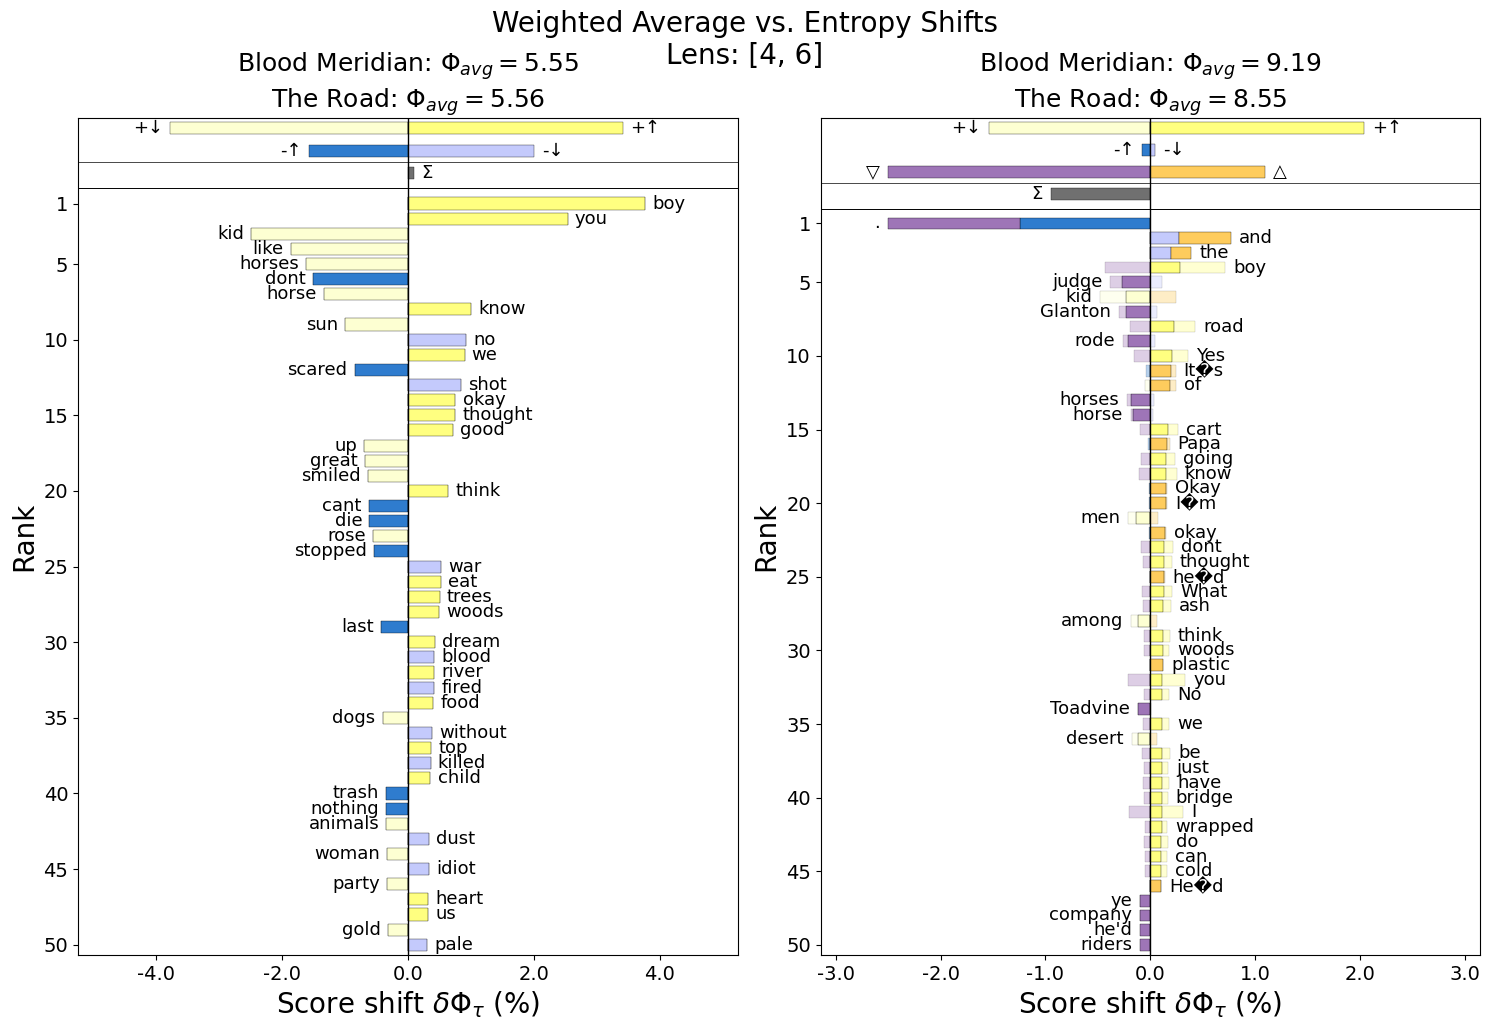
\includegraphics[width=\linewidth]{figures/21_1_a.png}
    \end{center}
    \clearpage
    
    The lensing interval used here is $[3,7]$, 
    using a reference value equal to the average happiness of lensed $\texta (5.266)$

    \begin{center}
        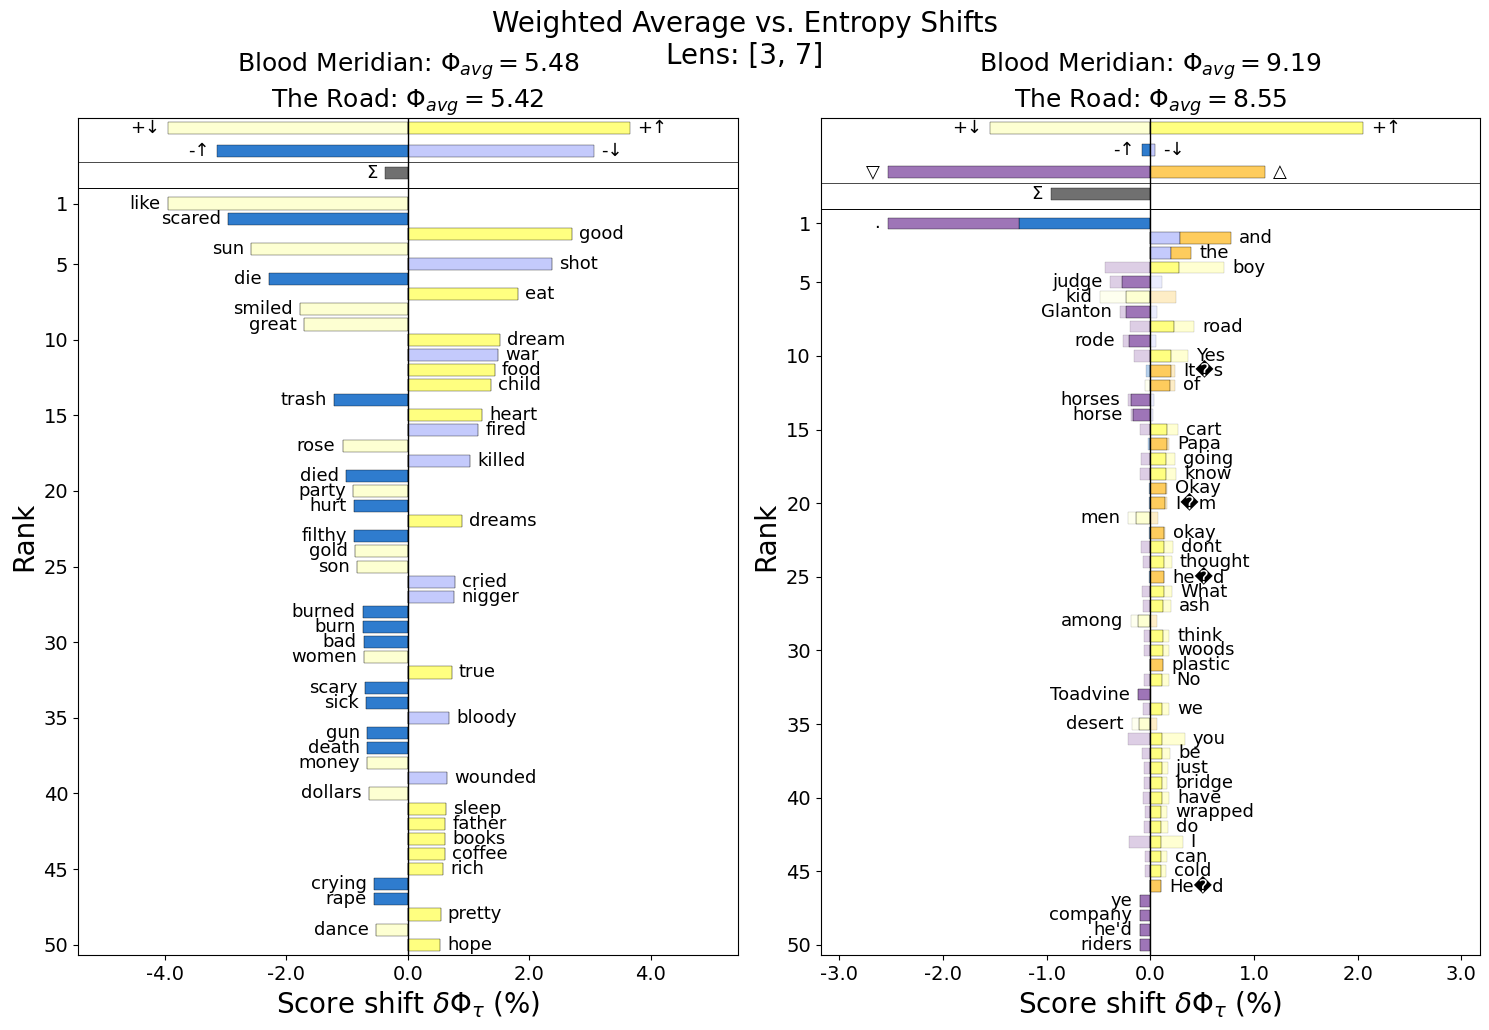
\includegraphics[width=\linewidth]{figures/21_1_a2.png}
    \end{center}

  \item 
    % Interpret the word shift. Does what you see make sense?
    % Are there any surprises?
    % Are some words being used in what the average person might not think is their primary meaning?
    % For example, ``crying'' in Moby Dick means yelling, and ``sick'' can mean ``awesome.''
    The results here make sense with respect to McCarthy's diction.
    It is important to note, however, that words which may generally have a "happy" connotation do not in the context of these works.

    For example, "party", "gold", "money", "dollars", and "dance" are often used in the context of a party of bandits, dancing over a slain person, or the seizing of material objects.

    The sentiment assigned to "like" is inappropriate in terms of McCarthy's diction, as it is often used to portray a simile. It would be nice if there were things in the novel which were objectively likeable, however it is like you are looking through a window where native peoples are beheaded for dollars. Needless to say, there is not much like the unflinching violence portrayed in $\texta$

    The only surprise, for me at least, is that $\texta$ is more gruesome than I remembered. While $\textb$ does not spare any details with respect to the brutality of life, there is a sense of hope portrayed by the author which is made evident in these comparisons.

    We see how narrowing the lens from $\pm 2$ to $\pm 1$
    
  \item
    % Produce a word shift comparing text $\texta$ relative to text $\textb$.
    % Use the average happiness of text $\textb$ as the baseline.
    Sticking with a reference value of $[3, 7]$ and using happiness average of $\textb (\Phi_{avg} = 5.280)$, but swapping the positions of $\texta$ and $\textb$ we have the figure below:

    \begin{center}
        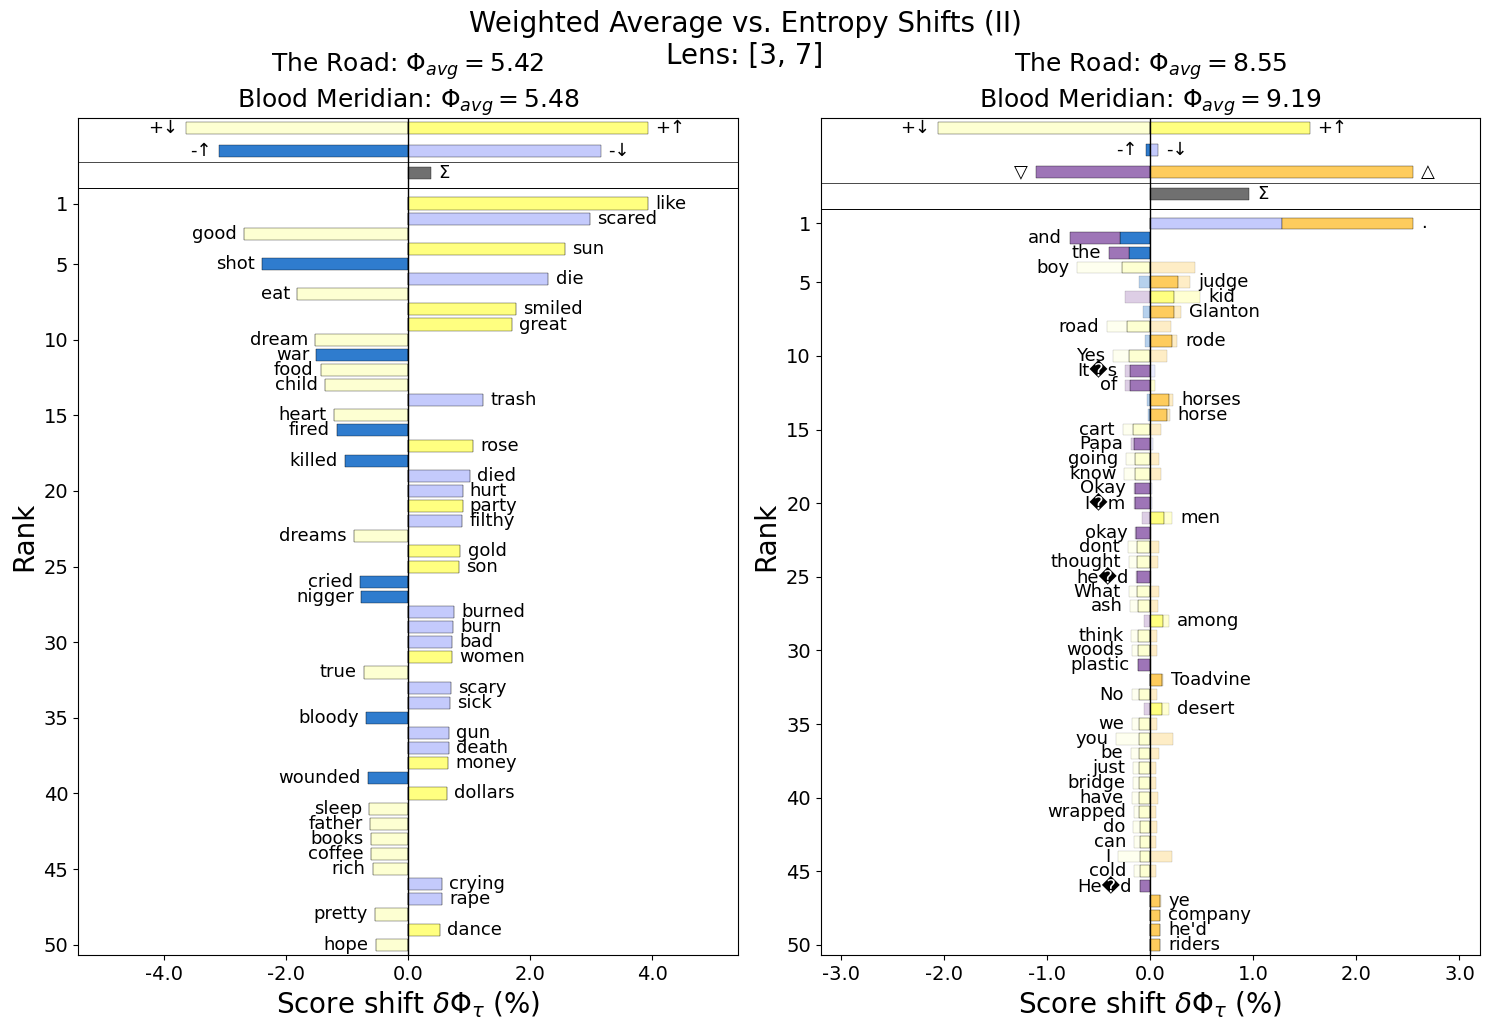
\includegraphics[width=\linewidth]{figures/21_1_c.png}
    \end{center}
    
  \item
    % Comment on any asymmetries you see (the basic word shifts we use are asymmetric).
    Let's start with the less than happy words identified for each.

    $\texta$ has 15 of the 23 negative words within the top 50 contributing words for weighted average shift.

    The scale of the frequency distributions with respect to their contributions towards the weighted average shift is greater in the $\texta$ direction (see $\Sigma$).
    \clearpage
    
  \item
    % Produce a word shift comparing text $\texta$ relative to text $\textb$.
    % Now use 5 as the baseline reference score (neutral on the happiness-sadness spectrum of 1--9).
    The top figure uses a reference value of 5, while the bottom figure is the first real figure, re-presented as a reference for the rhetor's relief from readjustment.
    
    \begin{center}
        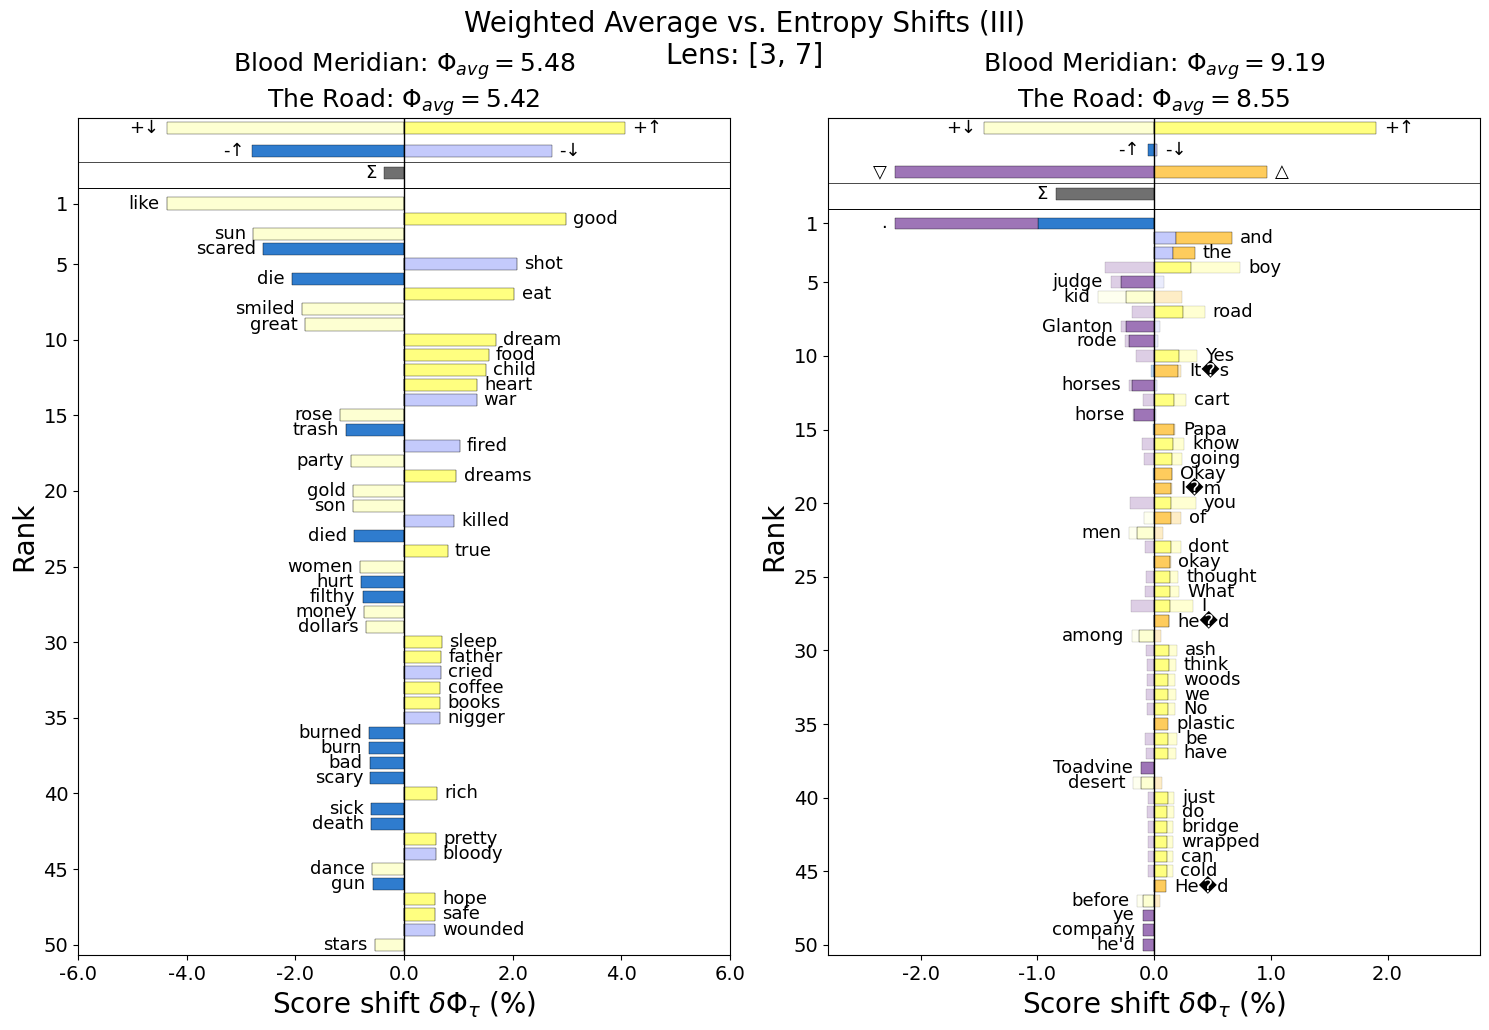
\includegraphics[width=\linewidth]{figures/21_1_e.png}
        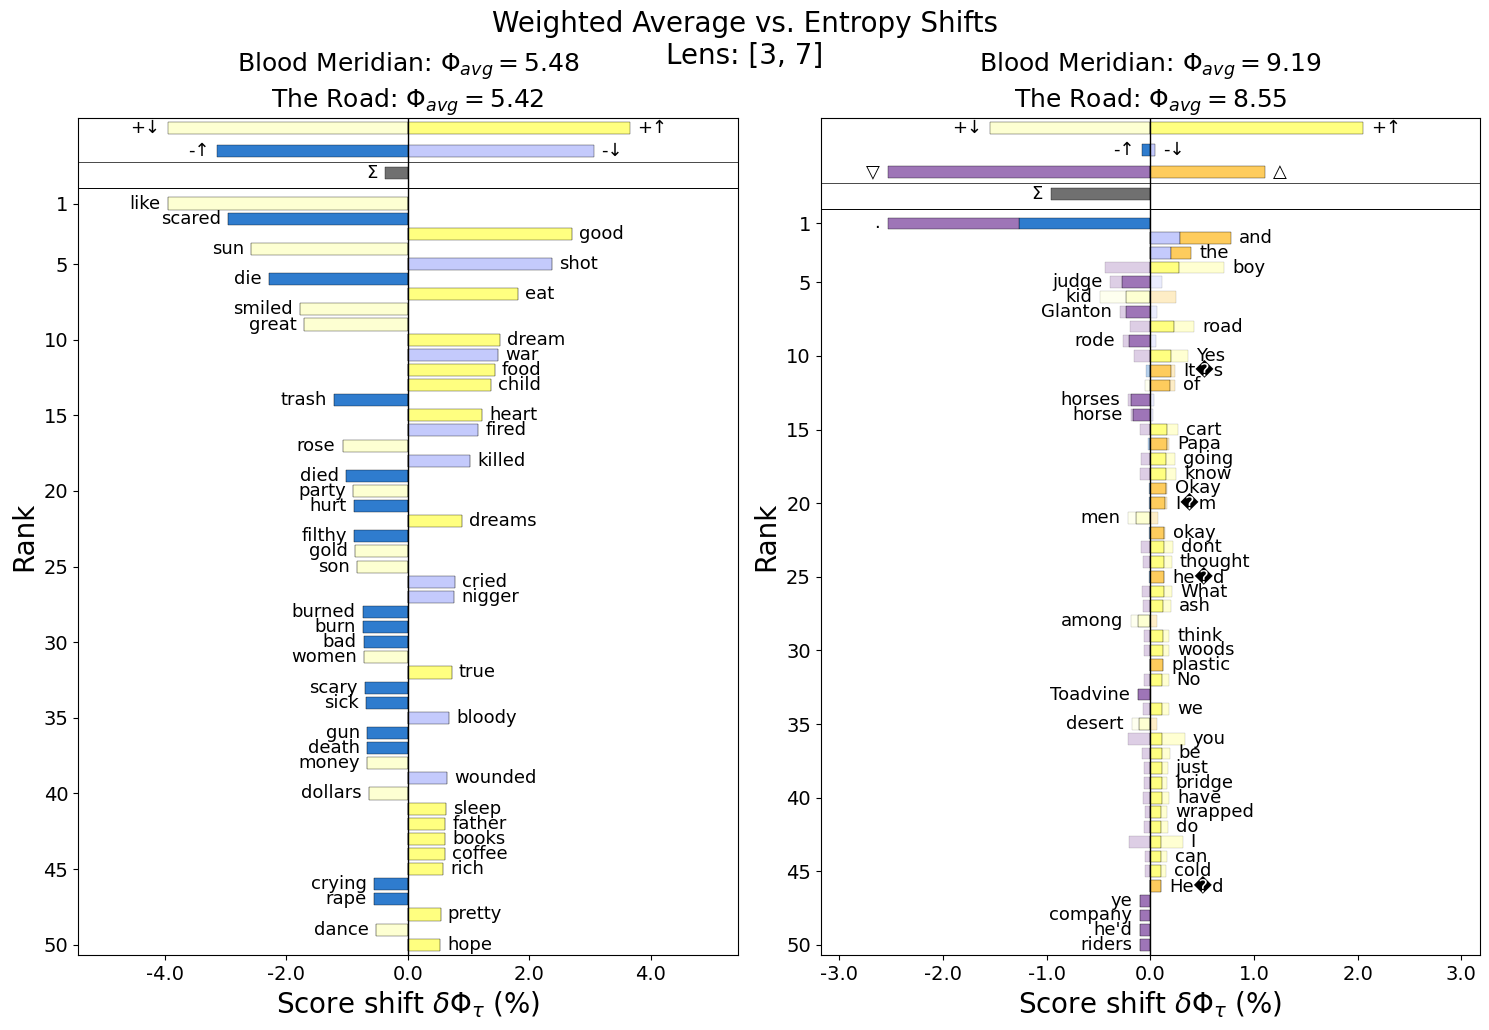
\includegraphics[width=\linewidth]{figures/21_1_a2.png}
    \end{center}
    
  \item
    % Compared to your first word shift, how interpretable is this one?

    Given that the average happiness of both texts is not significantly distant from 5, we do not see any startling changes.

    However, we do notice some of the more neutral words shifted lower (burned, burn, bad, women, etc.) which is to be expected if we are pretending that the happiness of these  words are not relative to the (con)text.

    I would say that they are both easily interpretable, understanding that the dictionary used to define the lexical happiness is neither exhaustive, nor is it necessarily appropriate to extend beyond the context of the relative comparisons that we have done thus far.

    In choosing the more appropriate reference value, we should err on the side of using the mean score of our reference text, as it is what we want to compare against.
    
  \end{enumerate}

   \solutionend

For additional viewing pleasure:

\begin{center}
    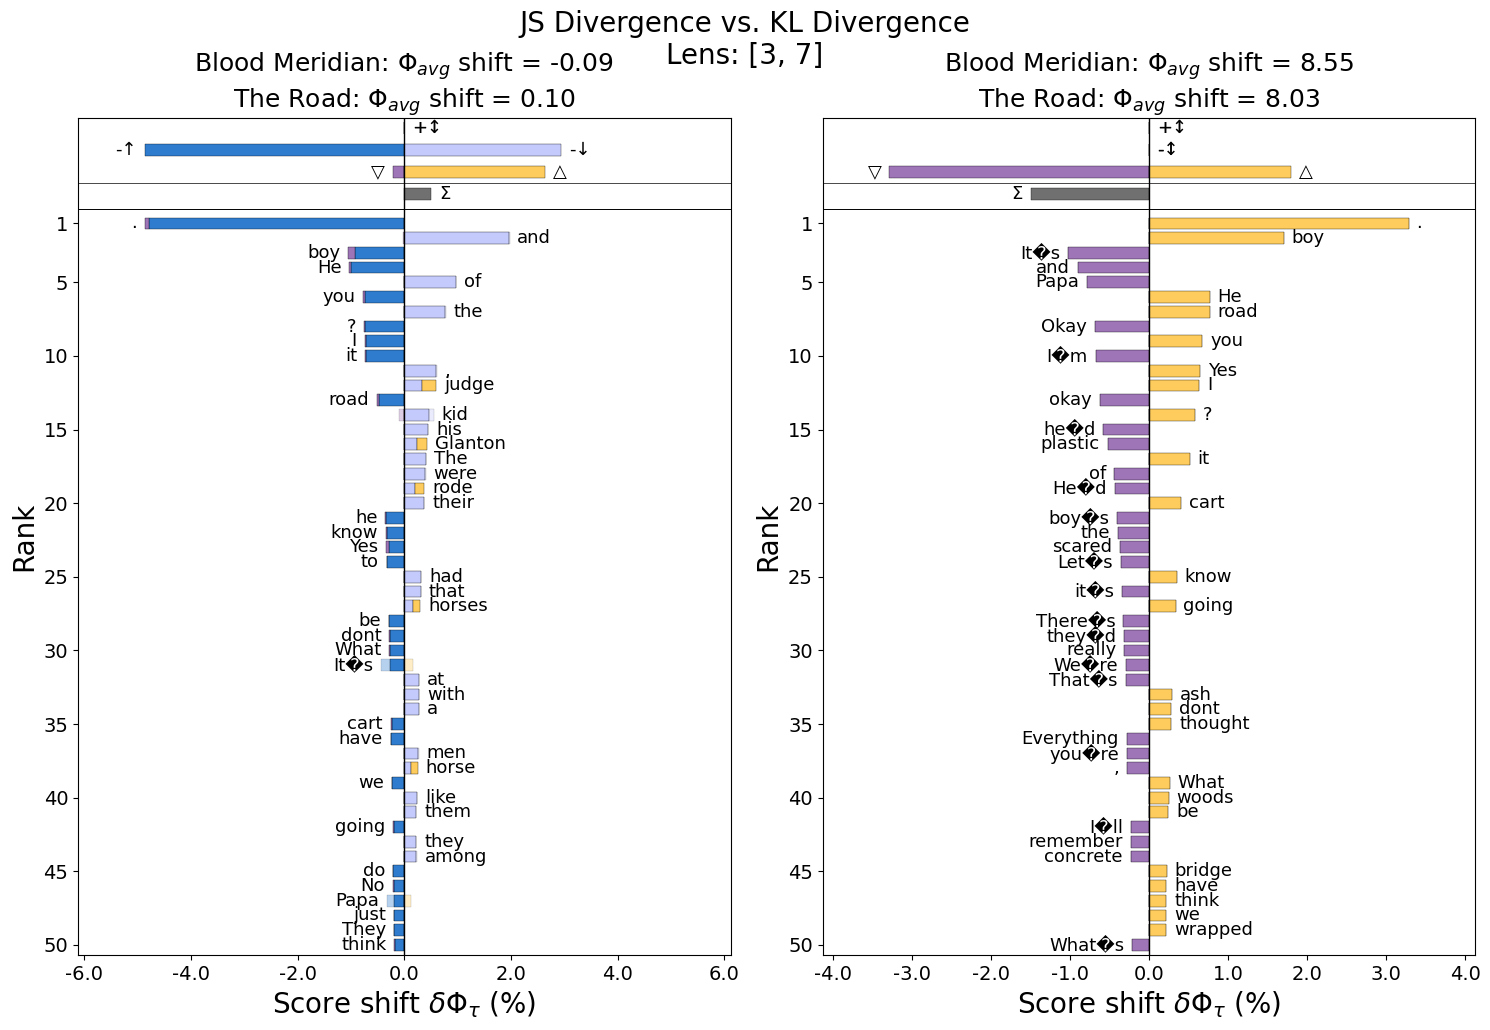
\includegraphics[width=\linewidth]{figures/jsd_kld.png}
\end{center}

\end{enumerate}




    
    \bibliographystyle{unsrtabbrv}
\bibliography{everything}


\end{document}
